\section{Main Result}
Stopping refinement need not mean discarding the triangles' remaining
information. Two neighboring hypotenuses also tell us how the average
slope changes across their shared vertex. If that change nearly exhausts
an independently known bound on slope variation, little freedom remains
for the smooth arc between the samples. We can turn this observation into
an explicit error certificate at the existing sampling scale.

\notesubsection{Angles and reconstruction}
Let $f\in C^2([u-h,u+h])$, $h>0$, and suppose $|f''|\le M$ for a
known $M>0$. Write $I_1=[u-h,u]$, $I_2=[u,u+h]$ and
$c_1=u-h/2$, $c_2=u+h/2$. The measured slopes are
\begin{equation}
 m_1=\frac{f(u)-f(u-h)}h=\tan\theta_1,\qquad
 m_2=\frac{f(u+h)-f(u)}h=\tan\theta_2,
\end{equation}
where the signed angles lie in $(-\pi/2,\pi/2)$. Set $s=1$ when
$m_2\ge m_1$ and $s=-1$ otherwise, and define
\begin{equation}\label{eq:deficit}
 D=Mh-|m_2-m_1|,\qquad q_i(x)=m_i+sM(x-c_i),\qquad
 \widehat L=\sum_{i=1}^2\int_{I_i}\sqrt{1+q_i(x)^2}\,dx.
\end{equation}
Each $q_i$ has the measured mean slope and changes at the largest
permitted rate in the observed direction. Integrating it reconstructs
a quadratic arc through that cell's endpoints. These arcs meet in
position, with derivative jump of magnitude $D$ at their shared vertex.

\noindent\textit{For every graph satisfying these assumptions,}
\begin{equation}\label{eq:main}
 \boxed{0\le D\le Mh,\qquad
 |L_{12}-\widehat L|\le2hD
 =2h\bigl(Mh-|\tan\theta_2-\tan\theta_1|\bigr),}
\end{equation}
\textit{where $L_{12}$ is its length on the two cells. If $D=0$, then
$f''=sM$ throughout, the three sampled values determine the graph
uniquely, and $L_{12}=\widehat L$.}

The estimator requires only elementary functions. With
$H(z)=\tfrac12[z\sqrt{1+z^2}+\asinh z]$, substitution gives
\begin{equation}\label{eq:evaluation}
 \widehat L=\frac1M\sum_{i=1}^2
 \bigl[H(m_i+Mh/2)-H(m_i-Mh/2)\bigr].
\end{equation}
This holds for either sign $s$. If $M=0$, the graph is affine and its
chord length is exact.

The reconstruction gives a concrete interpretation of the correction.
A chord replaces all slopes in its cell by their mean. The functions
$q_i$ restore slope variation while preserving the same endpoints.
Because $G(z)=\sqrt{1+z^2}$ is convex, each reconstructed arc is at
least as long as its chord. The uncertainty is how closely this
reconstructed variation follows the actual curve. Equation
\eqref{eq:main} controls that uncertainty using the observed turn.

The angles enter through their slopes $\tan\theta_i$, since the
sampling intervals have equal horizontal width. In a smooth graph the
slope changes continuously, whereas the chords record successive cell
averages. Their difference measures the integrated change that must
occur between those cells. When it reaches the permitted maximum,
equality leaves precisely the quadratic reconstruction.

\notesubsection{Proof}
To prove this, write $p=f'$. By the fundamental theorem of calculus,
each chord slope is the average of $p$ over its cell. Moving the
averaging interval one step to the right gives
\[
 m_2-m_1=\frac1h\int_{u-h}^{u}[p(x+h)-p(x)]\,dx,
 \qquad |p(x+h)-p(x)|\le Mh.
\]
Thus $|m_2-m_1|\le Mh$, establishing the stated range of $D$.
To measure departure from the reconstructed slope, remove its maximal
linear trend by putting
$r(x)=sp(x)-M(x-u)$. Since $r'=sf''-M\le0$, $r$ is nonincreasing.
Its cell averages satisfy
\[
 \bar r_1=sm_1+Mh/2,\qquad \bar r_2=sm_2-Mh/2,
 \qquad \bar r_1-\bar r_2=D.
\]
With $r_0=r(u)$, monotonicity gives $r\ge r_0$ on $I_1$ and
$r\le r_0$ on $I_2$, so
\[
 \sum_i\int_{I_i}|r-r_0|\,dx
 =h(\bar r_1-r_0)+h(r_0-\bar r_2)=hD,
 \qquad \sum_i h|\bar r_i-r_0|=hD.
\]
These identities use the shared vertex to control both cells together.
The first measures departure from $r_0$ inside the cells, and the second
measures how far their averages lie from that same value. Since
$s(p-q_i)=r-\bar r_i$, the triangle inequality gives
\[
 \sum_i\int_{I_i}|p-q_i|\,dx
 \le\sum_i\int_{I_i}|r-r_0|\,dx
       +\sum_i h|\bar r_i-r_0|.
\]
Consequently,
\begin{equation}\label{eq:slope-error}
 \sum_i\int_{I_i}|p-q_i|\,dx
 =\sum_i\int_{I_i}|r-\bar r_i|\,dx\le2hD.
\end{equation}
Finally $G(z)=\sqrt{1+z^2}$ satisfies
$|G'(z)|=|z|/\sqrt{1+z^2}\le1$. Therefore
\[
 |L_{12}-\widehat L|
 \le\sum_i\int_{I_i}|G(p)-G(q_i)|\,dx
 \le\sum_i\int_{I_i}|p-q_i|\,dx\le2hD.
\]
This proves the length bound. When $D=0$, the continuous nonnegative
integrands in \eqref{eq:slope-error} have zero integral, so $p=q_i$
on both cells. Thus $f''=sM$ throughout. Integrating twice gives
$f(x)=sMx^2/2+ax+b$, and the sampled values determine the remaining
affine coefficients. This proves the equality and uniqueness claims.

\notesubsection{A certified improvement}
The quantity $D$ measures the freedom left after the observed turn.
A slope change close to $Mh$ leaves little room to depart from the
maximal linear trend. Combining this information with the earlier
chord bound makes the improvement explicit. For
$C=h\sqrt{1+m_1^2}+h\sqrt{1+m_2^2}$, equations
\eqref{eq:bound} and \eqref{eq:main} imply
\begin{equation}\label{eq:intersection}
 \boxed{\max\{C,\widehat L-2hD\}\le L_{12}\le
 \min\{C+M^2h^3/12,\widehat L+2hD\}.}
\end{equation}
Its midpoint has absolute error at most half the interval width.
The width is at most the earlier $M^2h^3/12$, and the angular interval
alone has width $4hD$. Thus $D<M^2h^2/48$ suffices for a strict
reduction. The combined interval can also improve the bound when this
sufficient condition fails, as Figure 2 illustrates.

For a longer chain, group equal-width cells into disjoint adjacent pairs.
Writing $[A_j,B_j]$ for each pair's interval in \eqref{eq:intersection},
additivity gives
\[
 \left|L-\sum_j\widehat L_j\right|\le2h\sum_jD_j,
 \qquad \sum_jA_j\le L\le\sum_jB_j.
\]
An unpaired cell retains its chord bound. Using disjoint pairs ensures
that each arc is counted once. The midpoint of the summed interval has
absolute error at most half its width.

\notesubsection{The parabola and a quartic comparison}
For the parabola, even the three vertices $(-3,9),(0,0),(3,9)$ suffice
when $M=2$ is supplied independently. Here $h=3$, $m_1=-3$, $m_2=3$,
and $D=0$. The result forces $f''=2$ and then $f=x^2$, recovering
$L=19.494177517\ldots$ exactly from a chord sum of
$6\sqrt{10}=18.973665961\ldots$. At $k=3$ these are the two
triangles allowed by \eqref{eq:nk}, with legs $3$ and $9$.
The angular calculation recovers the missing $0.520511556\ldots$
without inserting another physical vertex.

To see the certificate away from equality, keep the three horizontal
sample coordinates and take $f_\varepsilon=x^2-\varepsilon x^4$ on
$[-3,3]$, with $0\le\varepsilon\le1/27$. Then
$f_\varepsilon''=2-12\varepsilon x^2\in[-2,2]$, so $M=2$ remains
valid. The slopes are $m_2=-m_1=3-27\varepsilon$, giving
$D=54\varepsilon$ and error radius $2hD=324\varepsilon$.
The vertical legs are at least $6$, retaining admissibility at $k=3$.

\par\medskip\noindent\begin{minipage}{\linewidth}
\centering
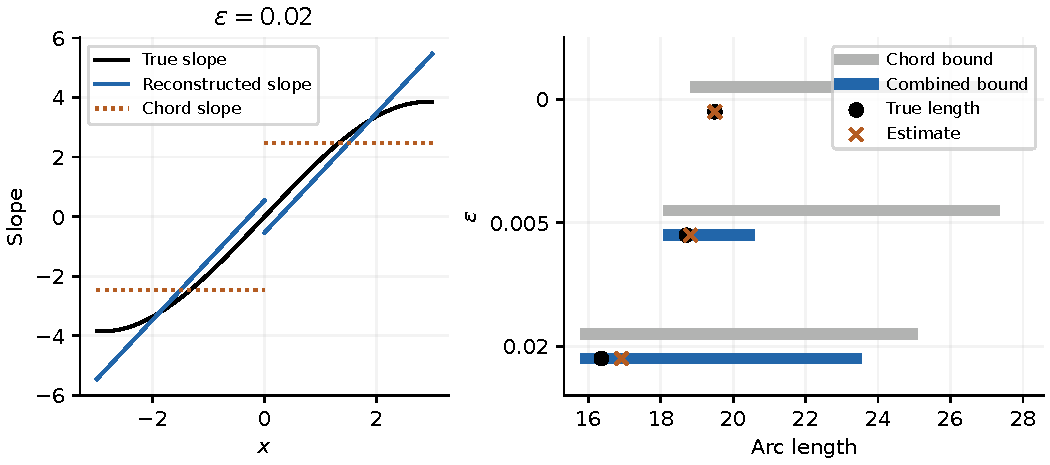
\includegraphics[width=.97\linewidth]{figures/angle_certificate.pdf}
\par\smallskip
\begin{minipage}{.95\linewidth}\small
\textbf{Figure 2.} Left, true, chord, and reconstructed slopes at
$\varepsilon=0.02$. Right, chord and combined bounds. Circles mark true
lengths and crosses mark $\widehat L$. Three samples suffice in each case.
\end{minipage}
\end{minipage}\par\medskip

\notesubsection{Interpretation and scope}
The independent bound $M$ restricts unresolved bending between vertices.
Here $M$ bounds the derivative of graph slope. Euclidean curvature is
$|f''|/(1+f'^2)^{3/2}$, so a curvature bound would need additional slope
information to supply this assumption.
A smooth bump can otherwise increase length while preserving every chord
angle. Setting $M=|m_2-m_1|/h$ from the samples gives only a necessary
lower bound and cannot justify exact recovery. Higher-order length
estimation has an established literature \cite{floater}. The contribution
developed here is inequality \eqref{eq:main}, with historical priority open.
